%package list
\documentclass{article}
\usepackage[top=3cm, bottom=3cm, outer=3cm, inner=3cm]{geometry}
\usepackage{graphicx}
\usepackage{url}
\usepackage{multirow}
%\usepackage{cite}
\usepackage{hyperref}
\usepackage{array}
\usepackage{multicol}
\newcolumntype{x}[1]{>{\centering\arraybackslash\hspace{0pt}}p{#1}}
\usepackage{natbib}
\usepackage{pdfpages}
\usepackage{multirow}
\usepackage{float}
\usepackage[normalem]{ulem}
\useunder{\uline}{\ul}{}




%%%%%%%%%%%%%%%%%%%%%%%%%%%%%%%%%%%%%%%%%%%%%%%%%%%%%%%%%%%%%%%%%%%%%%%%%%%%
%%%%%%%%%%%%%%%%%%%%%%%%%%%%%%%%%%%%%%%%%%%%%%%%%%%%%%%%%%%%%%%%%%%%%%%%%%%%
\newcommand{\csemail}{vmachacaa@unsa.edu.pe}
\newcommand{\csdocente}{Vicente Machaca Arceda}
\newcommand{\cscurso}{Algoritmos y Estructura de Datos}
\newcommand{\csuniversidad}{Universidad Nacional de San Agustín}
\newcommand{\csescuela}{Maestría en Ciencia de la Computación}
\newcommand{\cspracnr}{Final}
\newcommand{\cstema}{--}
%%%%%%%%%%%%%%%%%%%%%%%%%%%%%%%%%%%%%%%%%%%%%%%%%%%%%%%%%%%%%%%%%%%%%%%%%%%%
%%%%%%%%%%%%%%%%%%%%%%%%%%%%%%%%%%%%%%%%%%%%%%%%%%%%%%%%%%%%%%%%%%%%%%%%%%%%


\usepackage[english,spanish]{babel}
\usepackage[utf8]{inputenc}
\AtBeginDocument{\selectlanguage{spanish}}
\renewcommand{\figurename}{Figura}
\renewcommand{\refname}{Referencias}
\renewcommand{\tablename}{Tabla} %esto no funciona cuando se usa babel
\AtBeginDocument{%
	\renewcommand\tablename{Tabla}
}

\usepackage{fancyhdr}
\pagestyle{fancy}
\fancyhf{}
\setlength{\headheight}{30pt}
\renewcommand{\headrulewidth}{1pt}
\renewcommand{\footrulewidth}{1pt}
\fancyhead[L]{\raisebox{-0.2\height}{
\includegraphics[width=3cm]{Img/logo_unsa.jpg}}}
\fancyhead[C]{}
\fancyhead[R]{\fontsize{7}{7}\selectfont	\csuniversidad \\ \csescuela \\ \textbf{\cscurso} }
\fancyfoot[L]{MSc. Vicente Machaca}
\fancyfoot[C]{\cscurso}
\fancyfoot[R]{Página \thepage}







\begin{document}
	
	\vspace*{10px}
	
	\begin{center}	
		\fontsize{17}{17} \textbf{ Proyecto \cspracnr}
	\end{center}
	%\centerline{\textbf{\underline{\Large Título: Informe de revisión del estado del arte}}}
	%\vspace*{0.5cm}
	

	\begin{table}[h]
		\begin{tabular}{|x{4.7cm}|x{4.8cm}|x{4.8cm}|}
			\hline 
			\textbf{DOCENTE} & \textbf{CARRERA}  & \textbf{CURSO}   \\
			\hline 
			\csdocente & \csescuela & \cscurso    \\
			\hline 
		\end{tabular}
	\end{table}	
	
	
	\begin{table}[h]
		\begin{tabular}{|x{4.7cm}|x{4.8cm}|x{4.8cm}|}
			\hline 
			\textbf{PRÁCTICA} & \textbf{TEMA}  & \textbf{DURACIÓN}   \\
			\hline 
			\cspracnr & Algoritmos de ordenamiento  & 3 horas   \\
			\hline 
		\end{tabular}
	\end{table}
	
	
	\section{Datos de los estudiantes}
	Grupo: N° 8
	\begin{itemize}
		\item Integrantes: 
		\begin{itemize}
			\item Esai Josue Huaman Meza
			\item Alan Jerry Reyes Robles
			\item Jorge Luis Zegarra Guardamino
			\item Nestor Giraldo Calcinas Huaranga
		\end{itemize}		
	\end{itemize}
	
	
	
	
	
	
	\section{Introducción}
	
	Este proyecto final trata de la Clasificación de correos SPAM.

    Para esto se usará una parte del código utilizado en la práctica 04, para luego implementar un descriptor que para este caso será una bolsa de palabras.

    Para todo ello, el lenaguaje de programamción a usar será Java Script y Python.
	
El proyecto se encuentra en el siguiente enlace: \href{https://jzegarra100.github.io/KNN-JavaScript/}{Clasificador de Correos SPAM}.

El repositorio Github se encuentra en el siguiente enlace: \href{https://github.com/JZegarra100/KNN-JavaScript}{Clasificador SPAM}.

El video explicativo se encuentra en el siguiente enlace: \href{https://drive.google.com/file/d/1NfUwgwIfmOVS-lJdUTfy-Xi-OsMFhuhn/view?usp=sharing}{Clasificador de Correos SPAM - Grupo 8}.

El Descriptor hecho en Google Colab se encuentra en el siguiente enlace: \href{https://drive.google.com/file/d/1aKbI9XpST5vEPgCVhG_p8aBYKxg3QREd/view?usp=sharing}{Descriptor.py}.
	
	\section{SPAM}\label{sec:ejercicios}
	\begin{enumerate}
		\item \textbf{¿Qué es el SPAM?}

El spam es cualquier forma de comunicación no solicitada que se envía de forma masiva (correo electrónico masivo no solicitado, o UBE). Su forma más frecuente es un correo electrónico de publicidad enviado a un gran número de direcciones (correo electrónico de publicidad no solicitado, o UCE), pero el "spamming" también existe a través de menajes instantáneos, de texto (SMS), redes sociales o incluso mensajes de voz. Enviar spam es ilegal en la mayoría de jurisdicciones.

Una de las vías más comunes para propagar contenido no solicitado es a través de botnets, grandes redes de dispositivos "zombie" infectados. A veces los correos en cadena y fraudulentos también se consideran spam, aunque difieren en que en general se reenvían por gente con buenas intenciones.	

\begin{figure}[H]
\centering

\includegraphics[width=0.5\textwidth]{Img/spam.jpg}
\caption{Correos SPAM}
\end{figure}

\item \textbf{Tipos de SPAM}

\begin{itemize}
   \item SPAM por correos electrónicos
   \item SPAMming en buscadores
   \item SPAM telefónico
   \item SPAM en redes sociales
   \item SPAM a través de mensajería instantánea
\end{itemize}

\item \textbf{Origen de los Datos}

\begin{itemize}
   \item App store de Android
   \item Troyanos en Smartphones
   \item Redes sociales
   \item Fugas de datos
\end{itemize}

\item \textbf{Impacto del SPAM}

El SPAM está causando graves daños en el sistema mundial de comunicaciones. Los datos adicionales resultan en un esfuerzo de procesamiento considerablemente mayor. Además, la lectura y clasificación del spam es costosa, hay que comprar y mantener filtros de spam y se generan costes por cada byte transferido de spam, ya que los proveedores de servicios de Internet suelen cobrar por sus servicios en función del volumen de datos transferidos.

\end{enumerate}

\section{Marco Teórico}
\begin{enumerate}
		\item \textbf{Medidas para evitar el correo basura (SPAM)}

  A pesar de que no existen técnicas infalibles para protegerse del correo basura, los expertos en seguridad informática recomiendan una serie de acciones para reducir la cantidad de correo electrónico no deseado:

  \begin{itemize}
   \item Usar una imagen para la dirección de correo electrónico.
   \item En vez de poner el enlace a tu cuenta, usa una redirección (puede ser temporal o por un número de usos), y bórrala cuando recibas excesivos mensajes no deseados.
   \item Modificar la dirección para evitar el rastreo automático.
\end{itemize}

En los grupos de noticias y listas de correo:

\begin{itemize}
   \item No poner el remitente verdadero en las publicaciones enviados.
   \item Si el archivo de mensajes a la lista es visible desde web, cambiar las direcciones de remite por una imagen, ocultarlas, o escribirlas de forma que sea difícil reconocerla como tal para un programa.
\end{itemize}

\item \textbf{Proyectos y servicios contra el correo basura (SPAM)}

\begin{itemize}
   \item SPF: tecnología creada para verificar que los remitentes de los mensajes de correo son quienes dicen ser.
   \item DomainKeys: otra tecnología que sirve para lo mismo que SPF y que además asegura que los mensajes de correo electrónico no han sido modificados.
   \item SenderID: tecnología de Microsoft que pretende competir con SPF, incluso utilizando esas mismas siglas para una tecnología que en la práctica es distinta. En realidad, SenderID utiliza consultas DNS parecidas a SPF sólo como primer paso de su proceso, que involucra también filtros antispam basados en contenido. SenderID ha sido adoptado por Hotmail. En la práctica esto obliga a adoptar esta tecnología o verse excluido de esas direcciones, que suponen unos 260 millones de usuarios en todo el mundo. No obstante, los resultados de su tecnología, y/o otras medidas paralelas adoptadas, están causando serios problemas en dominios enteros en todo el mundo.
   \item Proyectos como el proyecto Harvester y el emailharvest recopilan las IP de generadores de basura para bloquearlas mediante una trampa. Ponen direcciones de correo que indican la dirección del remitente de correo masivo y cuando él envía un mensaje a esa dirección se sabe desde qué dirección fue capturada, con lo que puede filtrar al remitente.
   \item Redirecciones temporales.
\end{itemize}

\end{enumerate}

\section{Clasificador de Correos Electrónicos SPAM}

\begin{enumerate}
  \item \textbf{Utilizando KNN}
  
  El algoritmo k-nearest neighbor (KNN) es un método no paramétrico utilizado para clasificación y regresión. En lo que concierne a la clasificación, la idea básica  es  que,  dado  un  objeto del cual no conocemos su etiqueta de clase, a este se le asignará la etiqueta más común entre sus  vecinos más cercanos de acuerdo a una métrica de distancia.

  Para este proyecto usaremos el KNN implementado en una práctica anterior.

  \item \textbf{Utilizando una Bolsa de Palabras}

  Es un método que se utiliza en el procesado del lenguaje para representar documentos ignorando el orden de las palabras. En este modelo, cada documento parece una bolsa que contiene algunas palabras. Por lo tanto, este método permite un modelado de las palabras basado en diccionarios, donde cada bolsa contiene unas cuantas palabras del diccionario. En el campo de reconocimiento de objetos, se utiliza una idea similar para las representaciones de imágenes, es decir, una imagen puede ser tratada como un documento y las características extraídas de ciertos puntos de la imagen son consideradas palabras visuales. Las principales ventajas de utilizar este modelo es su facilidad de uso y su eficiencia computacional.

  \item \textbf{Utilizando Descriptor}

  Los descriptores de Python se crean para gestionar los atributos de diferentes clases que utilizan el objeto como referencia. En descriptores se utilizaron tres métodos diferentes que son getters, setters y delete. Si alguno de esos métodos está definido para un objeto, puede denominarse descriptor. Normalmente, Python usa métodos como getters y setters para ajustar los valores de los atributos sin ningún procesamiento especial. Es solo un sistema de almacenamiento básico. A veces, es posible que deba validar los valores que se asignan a un valor. Un descriptor es un mecanismo detrás de propiedades, métodos, métodos estáticos, métodos de clase y super.

\end{enumerate}

\section{Implementación}

  Este proyecto se desarrolla utilizando los lenguajes Python y Java Script, los cuales se pueden encontrar en el siguiente repositorio Github \href{https://github.com/JZegarra100/KNN-JavaScript}{Clasificador SPAM}., y se obtienen las siguientes imágenes.

\section{Resultados}

    \begin{enumerate}
    
        \item \textbf{Descriptor}

\begin{figure}[H]
\centering
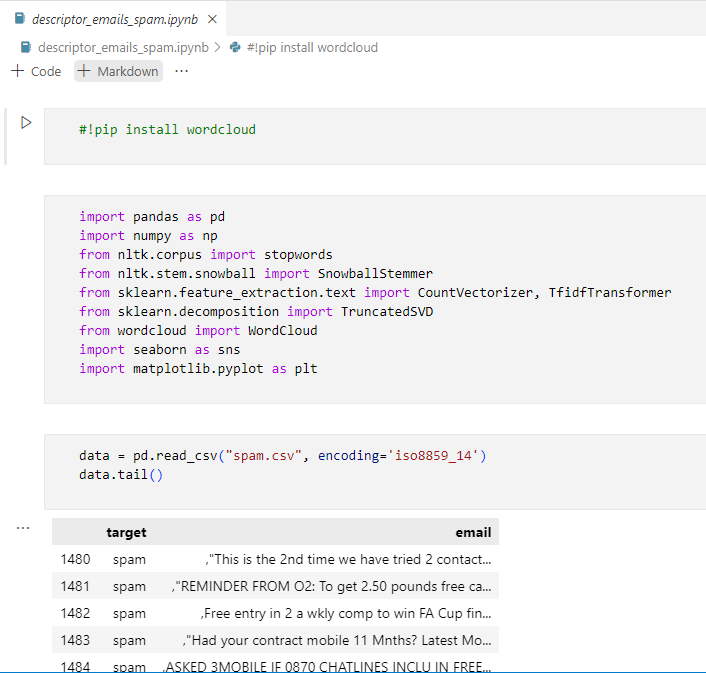
\includegraphics[width=0.95\textwidth]{Img/descriptor.png}
\caption{Descriptor}
\end{figure}

\item \textbf{Data de correos SPAM}

\begin{figure}[H]
\centering
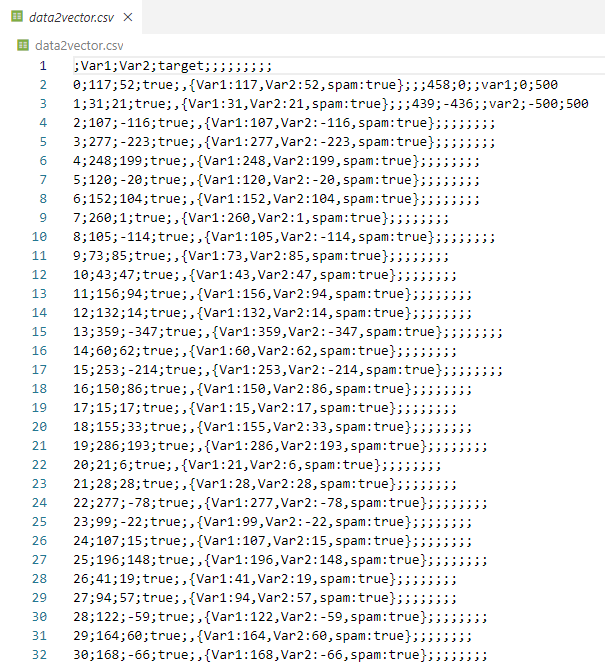
\includegraphics[width=1.15\textwidth]{Img/Correos SPAM.py.png}
\caption{Data Generado por el Descriptor (1476 datos)}
\end{figure}

\item \textbf{KNN}

\begin{figure}[H]
\centering
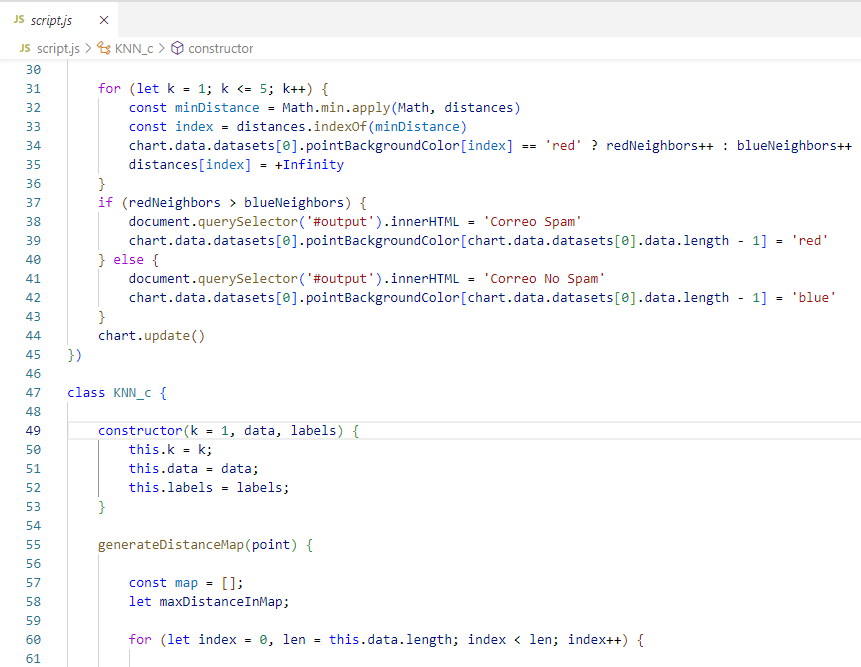
\includegraphics[width=1.1\textwidth]{Img/KNN.png}
\caption{KNN utilizado}
\end{figure}

\item \textbf{Index.html}

\begin{figure}[H]
\centering
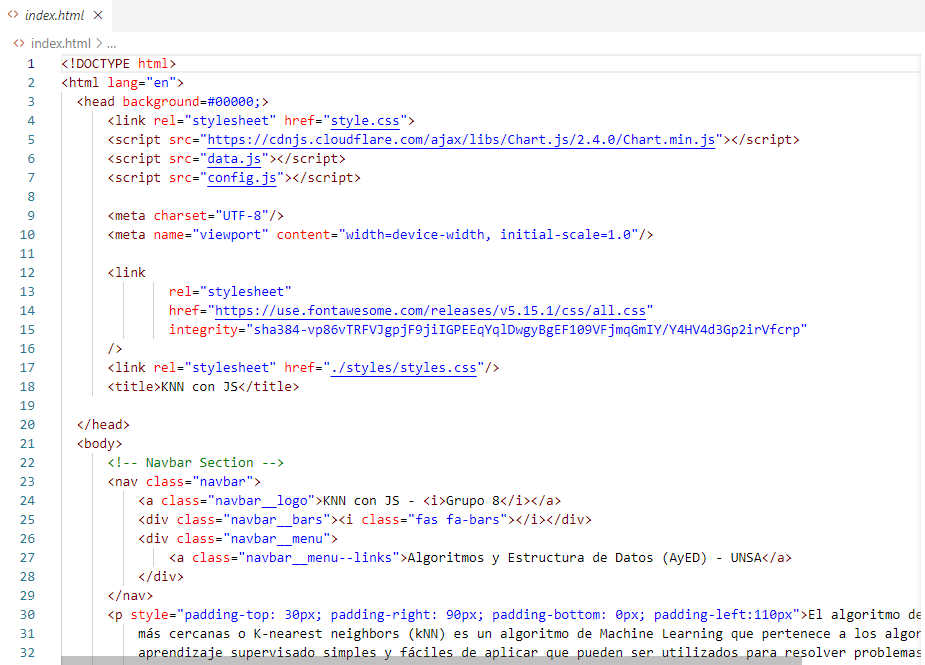
\includegraphics[width=1.1\textwidth]{Img/Index.png}
\caption{Index.html}
\end{figure}

\item \textbf{Visualización HTML}

\begin{figure}[H]
\centering
\includegraphics[width=1.1\textwidth]{Img/Visualización Index.png}
\caption{Visualización de pantalla}
\end{figure}

\section{Conclusiones}

\begin{itemize}
   \item El  filtrado  de  correo  no deseado  es  un  tema  importante  en  seguridad  de  red y  actualmente  las  técnicas  de aprendizaje automático brindan una alternativa muy interesante y eficiente para resolver este tipo de problemas.
   \item El Knn es un algoritmo de aprendizaje supervisado, a partir de un juego de datos inicial, su objetivo será el de clasificar correctamente todas las instancias nuevas. El juego de datos típico de este tipo de algoritmos está formado por varios atributos descriptivos y un solo atributo objetivo.
   \item El Knn es sensible a la variable k, que con valores distintos de k podemos obtener resultados también muy distintos sobretodo en los bordes de la clasificacion. La métrica de similitud utilizada (el descriptor a usar), puesto que esta influirá, fuertemente, en las relaciones de cercanía que se irán estableciendo en el proceso de construcción del algoritmo.

\end{itemize}

    

    \end{enumerate}
	
	%\clearpage
	%\bibliographystyle{apalike}
	%\bibliographystyle{IEEEtranN}
	%\bibliography{bibliography}
		
	
\end{document}